
\documentclass[ 
	% -- opções da classe memoir --
	article,			% indica que é um artigo acadêmico
	11pt,				% tamanho da fonte
	oneside,			% para impressão apenas no verso. Oposto a twoside
	a4paper,			% tamanho do papel. 
	% -- opções da classe abntex2 --
	%chapter=TITLE,		% títulos de capítulos convertidos em letras maiúsculas
	%section=TITLE,		% títulos de seções convertidos em letras maiúsculas
	%subsection=TITLE,	% títulos de subseções convertidos em letras maiúsculas
	%subsubsection=TITLE % títulos de subsubseções convertidos em letras maiúsculas
	% -- opções do pacote babel --
	english,			% idioma adicional para hifenização
	brazil,				% o último idioma é o principal do documento
	]{abntex2}


% --- 
% PACOTES
% ---

% ---
% Pacotes fundamentais 
% ---
\usepackage{cmap}				% Mapear caracteres especiais no PDF
\usepackage{lmodern}			% Usa a fonte Latin Modern
\usepackage[T1]{fontenc}		% Selecao de codigos de fonte.
\usepackage[utf8]{inputenc}		% Codificacao do documento (conversão automática dos acentos)
\usepackage{indentfirst}		% Indenta o primeiro parágrafo de cada seção.
\usepackage{nomencl} 			% Lista de simbolos
\usepackage{color}				% Controle das cores
\usepackage{graphicx}			% Inclusão de gráficos
\usepackage{csvsimple}
\usepackage{epstopdf}
\usepackage{multirow}
%\usepackage[nolists,tablesfirst]{endfloat}
% ---
		
\usepackage{amsmath}		
		
		
% ---
% Pacotes adicionais, usados apenas no âmbito do Modelo Canônico do abnteX2
% ---
\usepackage{lipsum}				% para geração de dummy text
% ---
		
% ---
% Pacotes de citações
% ---
\usepackage[brazilian,hyperpageref]{backref}	 % Paginas com as citações na bibl
\usepackage[alf]{abntex2cite}	% Citações padrão ABNT
% ---

% ---
% Configurações do pacote backref
% Usado sem a opção hyperpageref de backref
\renewcommand{\backrefpagesname}{Citado na(s) página(s):~}
% Texto padrão antes do número das páginas
\renewcommand{\backref}{}
% Define os textos da citação
\renewcommand*{\backrefalt}[4]{
	\ifcase #1 %
		Nenhuma citação no texto.%
	\or
		Citado na página #2.%
	\else
		Citado #1 vezes nas páginas #2.%
	\fi}%
% ---

% ---
% Informações de dados para CAPA e FOLHA DE ROSTO
% ---
\titulo{Relatório de atividades: Uso do classificador Bayesiano} 
\autor{David Clifte\thanks{cliftedavid@gmail.com}}
\local{Brasil}
\data{2015, v-1.0}
% ---

% ---
% Configurações de aparência do PDF final

% alterando o aspecto da cor azul
\definecolor{blue}{RGB}{41,5,195}

% informações do PDF
\makeatletter
\hypersetup{
     	%pagebackref=true,
		pdftitle={\@title}, 
		pdfauthor={\@author},
    	pdfsubject={Modelo de artigo científico com abnTeX2},
	    pdfcreator={LaTeX with abnTeX2},
		pdfkeywords={abnt}{latex}{abntex}{abntex2}{atigo científico}, 
		colorlinks=true,       		% false: boxed links; true: colored links
    	linkcolor=blue,          	% color of internal links
    	citecolor=blue,        		% color of links to bibliography
    	filecolor=magenta,      		% color of file links
		urlcolor=blue,
		bookmarksdepth=4
}
\makeatother
% --- 

% ---
% compila o indice
% ---
\makeindex
% ---

% ---
% Altera as margens padrões
% ---
\setlrmarginsandblock{4cm}{4cm}{*}
\setulmarginsandblock{4cm}{4cm}{*}
\checkandfixthelayout
% ---

% --- 
% Espaçamentos entre linhas e parágrafos 
% --- 

% O tamanho do parágrafo é dado por:
\setlength{\parindent}{1.3cm}

% Controle do espaçamento entre um parágrafo e outro:
\setlength{\parskip}{0.2cm}  % tente também \onelineskip

% Espaçamento simples
\SingleSpacing

% ----
% Início do documento
% ----
\begin{document}

% Retira espaço extra obsoleto entre as frases.
\frenchspacing 

% ----------------------------------------------------------
% ELEMENTOS PRÉ-TEXTUAIS
% ----------------------------------------------------------

%---
%
% Se desejar escrever o artigo em duas colunas, descomente a linha abaixo
% e a linha com o texto ``FIM DE ARTIGO EM DUAS COLUNAS''.
% \twocolumn[    		% INICIO DE ARTIGO EM DUAS COLUNAS
%
%---
% página de titulo
\maketitle

% resumo em português
\begin{resumoumacoluna}
 Este trabalho apresenta os resultados obtidos ao aplicar o classificador
 bayessiano e submete-lo a 5 diferentes funções de densidade de probabilidade.
 Para a verificação da acurácia bem como das regiões de decisão são
 apresentados os resultados obtidos com três base de dados diferentes.
 A implementação foi feita no Matlab\texttrademark
 
 
 \vspace{\onelineskip}
 
 \noindent
 \textbf{Palavras-chaves}: Bayes. Reconhecimento de padrões.
\end{resumoumacoluna}

% ]  				% FIM DE ARTIGO EM DUAS COLUNAS
% ---

% ----------------------------------------------------------
% ELEMENTOS TEXTUAIS
% ----------------------------------------------------------
\textual

% ----------------------------------------------------------
% Introdução
% ----------------------------------------------------------
\section*{Introdução}


% ---------------------------------------------------------- Seção de
% explicações ----------------------------------------------------------
\subsection{Estimativa de função de densidade de probabilidade}
A estimativa da distribuição de dados é importante pois permite utilizar uma
representação compacta dos dados e ainda sim mater as informações mais
relevantes da base. Existem basicamente três abordagens para estimar a função de
densidade de probabilidade de um sinal: paramétrica, não- paramétrica e
semiparamétrica. O sucesso destas representações dependem do modelo que tem sido definido.

\subsubsection{Método não paramétrico}
Os métodos não-paramétricos não fazem nenhuma consideração da distribuição de proba-
bilidade dos dados. Em geral, estes métodos se caracterizam por conseguir uma estimativa ade-
quada para qualquer conjunto de dados que recebem como entrada.


\subsubsection{Método paramétrico}
A abordagem paramétrica é geralmente usada quando a distribuição dos dados é conhe-
cida antecipadamente ou quando os dados são simples de forma que permitam ser modelados
usando uma distribuição conhecida, por exemplo gaussiana, Gamma, Laplace, etc

\subsubsection{Método semi-paramétrico}
A abordagem semiparamétrica  combina a flexibilidade da abor- dagem
não-paramétrica e a eficiência na avaliação dos parâmetros da abordagem
paramétrica. Estes modelos utilizam um número de funções base que são sempre
menores que o conjunto de treinamento. O uso dos modelos semiparamétricos
baseados em gaussianas,GMM, tem se apresentado como uma ferramenta amplamente
usada na estimativa da PDF de qualquer sinal.


\subsection{Gaussian Misture Models}

\subsubsection{Introdução}
Considerando um conjunto de dados $X={x_1,x_2,\ldots,x_n}| x \in R$ , a PDF dos
dados pode ser aproximada por uma família $F$ de funções de distribuição de
probabilidades em R. Em algoritmos dedicados à estimativa da PDF, o problema é
encontrar a função de distribuição $f(x) \in F$ que melhor gere os dados de
entrada.

\begin{equation}
f(x,\Theta)=\sum^{k}_{k=1}P_kg(x,\mu_k,\sigma_k)
\end{equation}

$\Theta$ é o conjunto de parâmetros do conjunto de funções que devem ser
estimados durante a fase de treinamento. Desta forma para gaussiana temos

\begin{equation}
	\Theta=
	\begin{bmatrix}
		\mu_1 & \sigma_1 \\
		\ldots & \ldots \\
		\mu_k & \sigma_k 
	\end{bmatrix}
\end{equation}

$\Theta$ pode ser estimado utilizando o Algoritmo Maximização da Expectância
(EM). O algoritmo EM é um procedimento iterativo para estimar
os parâmetros de uma mistura de gaussianas.Cada iteração do algoritmo EM
consiste em dois processos: Expectância e Maximização.
Esta aproximação se consegue através do cálculo da probabilidade de perti-
nência de um ponto às funções de distribuições na fase de expectância. Na fase
de maximização são estimados os parâmetros que maximizam cada função de
distribuição, ponderadas com os valores calculados na fase de expectância.


Na figura \ref{fig:gmmIris} é apresentado o resultado da aproximação da base da
íris. São exibidas três das quatro combinações possíveis das características da
base, essas combinações são utilizadas para realizar o treinamento do GMM.



\begin{figure}
	\centering
	\begin{tabular}{ccc}

	  %Íris
	  \includegraphics[width=40mm]{matlab/gmm/iris/1-4/Functions.eps}
	  &
	  \includegraphics[width=40mm]{matlab/gmm/iris/1-4/resultPDF.eps}
	  &
	  \includegraphics[width=40mm]{matlab/gmm/iris/1-4/resultPDF3D.eps}
	  \\
	  
	  \includegraphics[width=40mm]{matlab/gmm/iris/2-4/Functions.eps}
	  &
	  \includegraphics[width=40mm]{matlab/gmm/iris/2-4/resultPDF.eps}
	  &
	  \includegraphics[width=40mm]{matlab/gmm/iris/2-4/resultPDF3D.eps}
	  \\
	  
	  \includegraphics[width=40mm]{matlab/gmm/iris/2-3/Functions.eps}
	  &
	  \includegraphics[width=40mm]{matlab/gmm/iris/2-3/resultPDF.eps}
	  &
	  \includegraphics[width=40mm]{matlab/gmm/iris/2-3/resultPDF3D.eps}
	  \\
	  	  
	  a) Conjunto de funções
	  &
	  b) f(x)
	  &
	  c) f(x) no $R^3$
	  \\
	\end{tabular}
	\caption{Resultados obtidos ao utilizar a mistura de gaussianas para modelar
	a base de dados da íris. Na primeira linha temos o resultado do treinamento
	utilizando as informações comprimento da sepala e largura da pétala. Na linha
	seguinte temos largura da sépala e da pétala e na terceira linha o comprimento
	da sépala e largura da pétala }
	\label{fig:gmmIris}
\end{figure}






\subsection{Base de dados da coluna vertebral}

Nessa base de dados os atributos são pelvic incidence, pelvic tilt, lumbar
lordosis angle, sacral slope, pelvic radius e grade of spondylolisthesis.
São 310 amostras onde 19,3 \% são pacientes com hernia, 48,3\% pacientes com
Spondylolisthesis e 32.2\% pacientes normais.

\subsection{Normalização e codificação}
\label{ss:normCodf} 
Após o carregamento da base foi realizado apenas a normalização dos dados e a
codificação dos rótulos. A normalização foi realizada separadamente para cada
atributo. Foi identificado o máximo e o mínimo do atributo $p$ e todos os
valores foram normalizados na faixa [0,1].

A codificação do rótulo foi feita no modelo 1-de-k(1-of-K ou one-hot encoding),
nesse modelo o rótulo é codificado em um vetor onde cada posição do
vetor representa uma classe. Nesse modelo para uma quantidade $m$ de classes
temos um vetor com $m$ posições e a classe $k$ é representada por um vetor
onde todas as outras posições diferentes de $k$ possuem o valor zero e a
posição $k$ possui o valor 1. Dessa forma as três classes possíveis da íris
foram codificadas em um vetor de 3 posições, onde a posição 1, 2 e 3
representam a classe setosa, versicolor e virgínica respectivamente. O mesmo foi
repetido para as bases da dermatologia e da coluna vertebral.


% %Gráfico em barra
% \subsection{Análise das características}
% \label{ss:analiCara}
% 
% \subsubsection{Base da íris}
% Na figura \ref{fig:charMatrix} é apresentada a matriz de características. 
% Essa matriz consiste de gráficos formados pelos pares de características
% combinadas.
% 
% Na diagonal principal é apresentado o histograma do atributo.
% Devido a natureza continua dos atributos do problema, pois o
% comprimento e largura da sépala e pétala podem assumir qualquer valor real O
% histograma foi obtido após a realização da quantização dos atributos.
% Cada atributo foi quantizado em 15 possíveis valores com faixas de mesma largura. A
% largura da faixa foi obtida da seguinte forma $(max_p - min_p)/15$, onde max e
% min são os valores máximos e mínimos do atributo $p$.
% 
% \begin{figure}[!htb] \centering
% 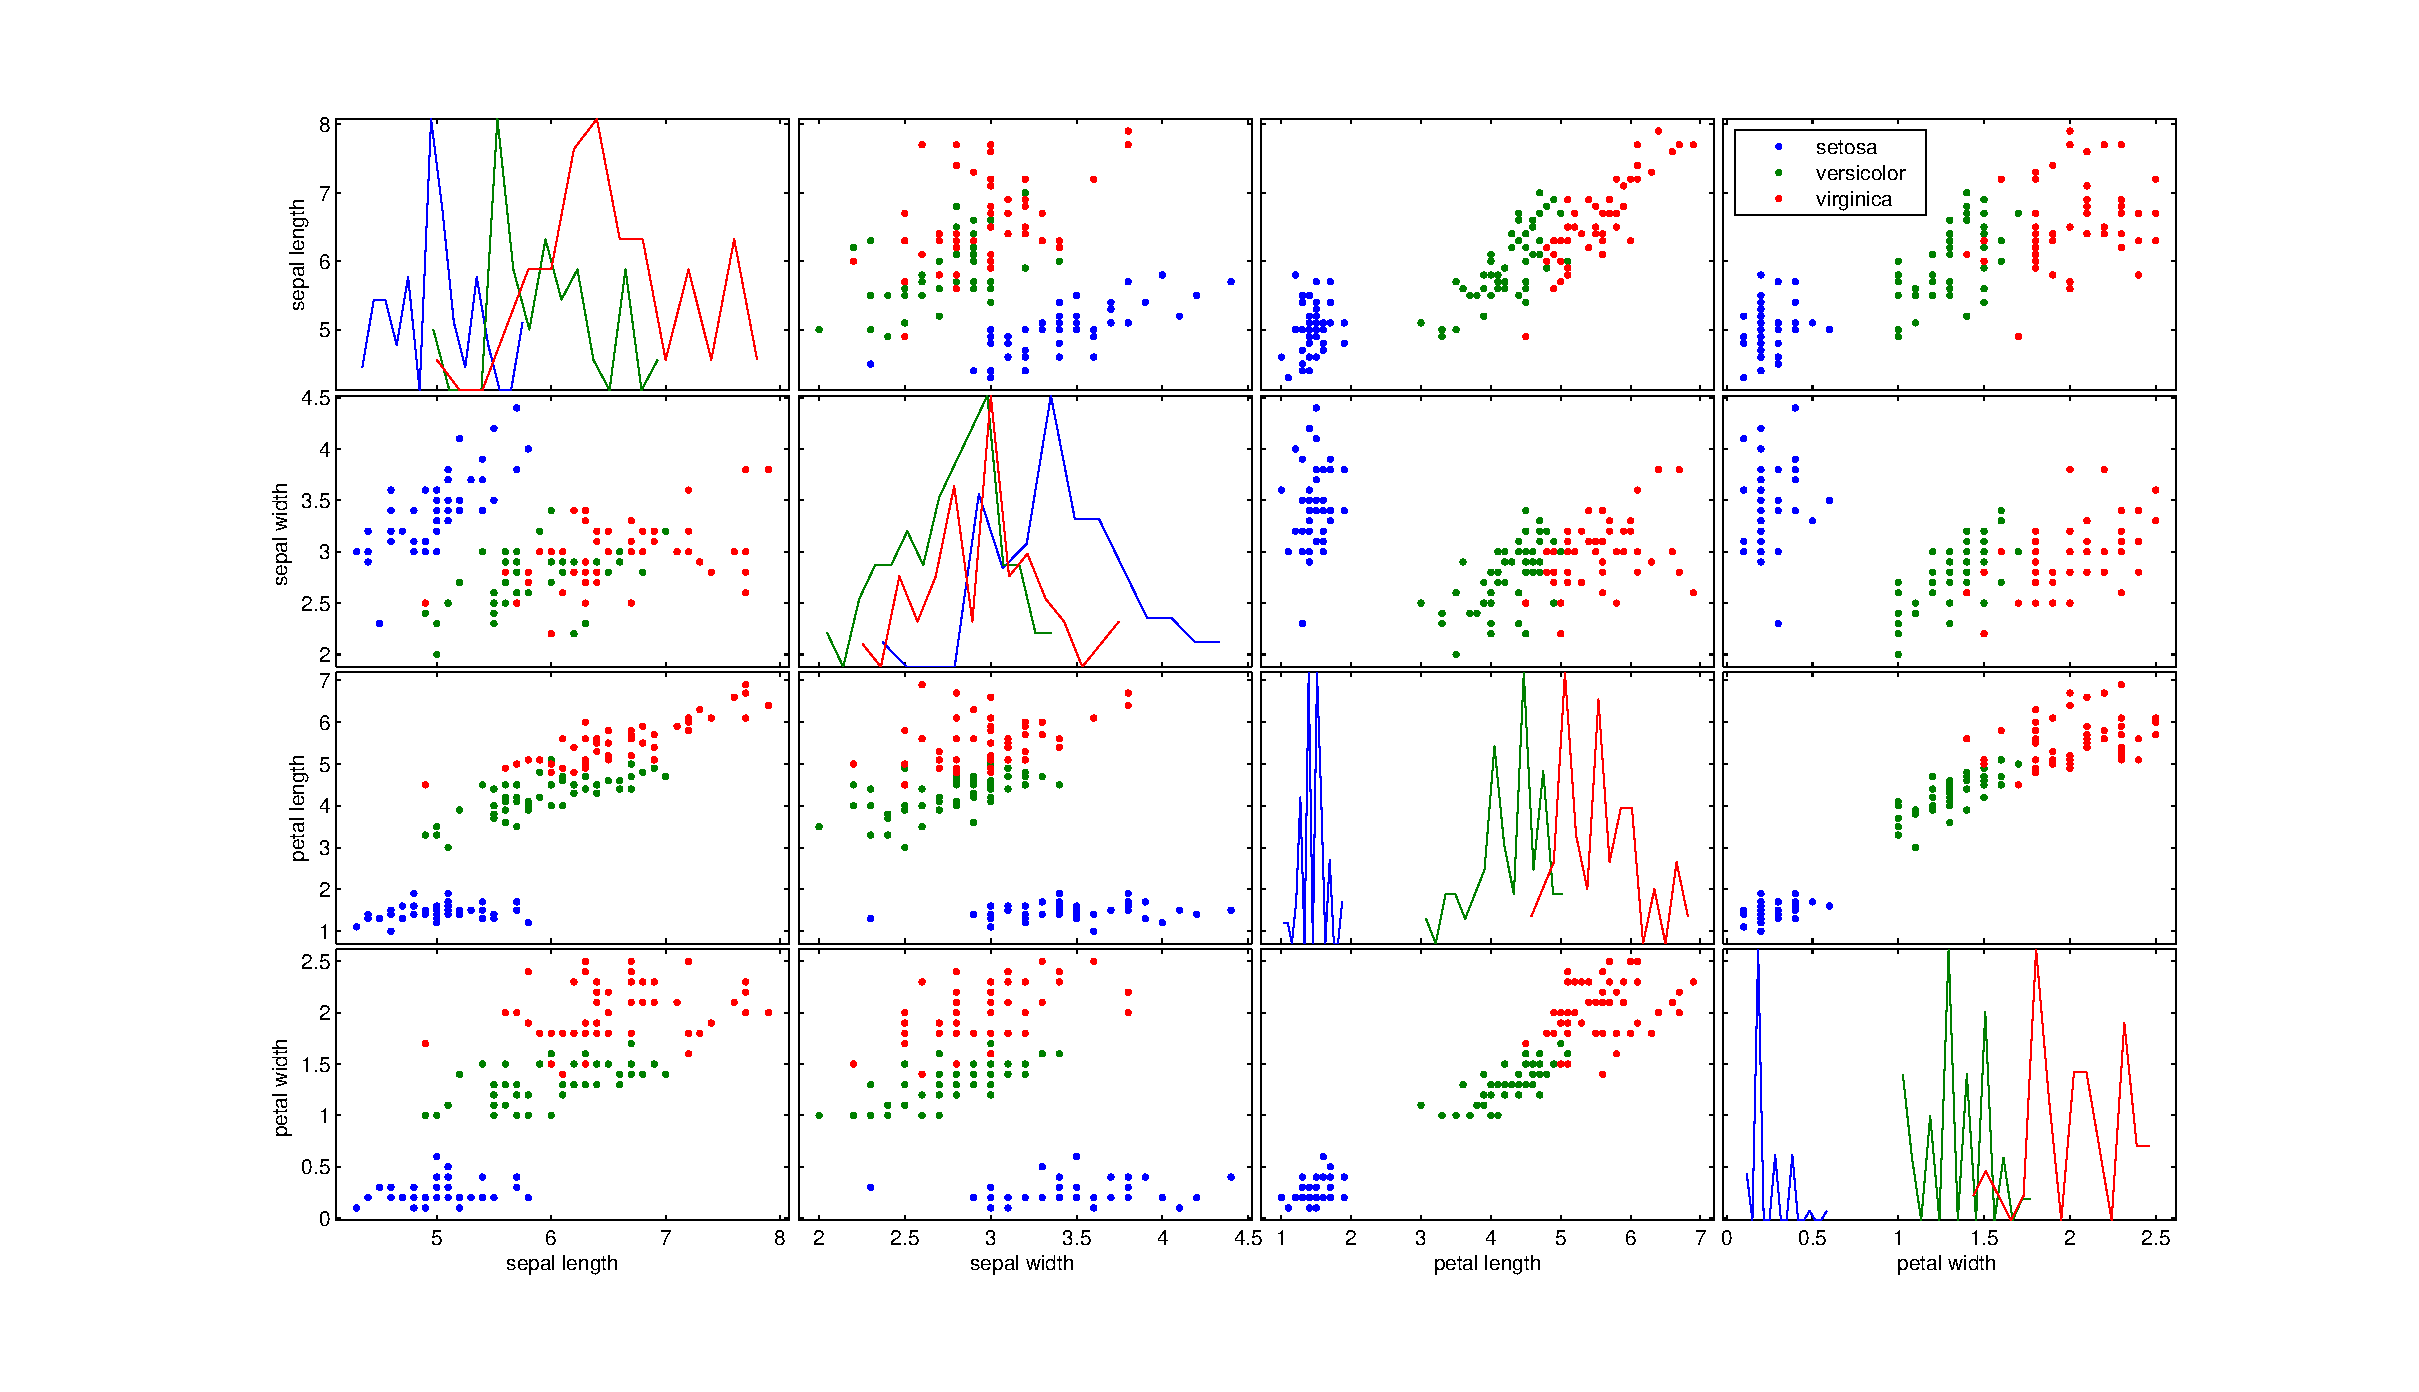
\includegraphics[width=\textwidth]{figuras/analiseIris_hist_scatterMatrix.eps}
% \caption{Matriz de características.}
% \label{fig:charMatrix}
% \end{figure}
% 
%  Podemos perceber que a classe setosa pode facilmente ser separada das outras
%  utilizando a largura ou o comprimento da pétala como variável. Nos histogramas
%  localizados na parte inferior isso pode ser verificado, pétalas com
%  comprimentos menores que 0,25 ou sépalas com largura menor que 0,3 de
%  comprimento são claramente da classe setosa.
%  Já para as duas outras características essa separação não é tão simples,
%  perceba a sobreposição dos histogramas em todos os atributos bem como a mistura
%  das classes nos gráficos de dispersão.
%  
%  \subsubsection{Base da coluna vertebral}
%  
%  \subsubsection{Base da dermatologia}


\section{Classificador de Bayes}

\subsection{Introdução}
Dada uma classificação entre M classes, o classificador de Bayes faz a seleção
de um dado $x$ com base na probabilidade de $w_i$ dado um $x$ , $P(w_i|x)$.
Assim temos:


\begin{equation}
	x \in w_i \iff P(w_i|x) \geq P(w_j|x) \forall i \neq j
\end{equation}

\subsection{Metodologia}
\label{ss:metAplbayes}
Na sessão \ref{ss:resultadosObtidos} são apresentados os resultados obtidos ao
aplicar o classificador de bayes utilizando como função de densidade
probabilidade a Gaussiana e as distâncias eclidiana e de mahanalanobis. Para
todos os conjuntos de dados os testes foram realizados sobre uma partição de 25\% do total de dados, escolhida de forma
aleatória para cada repetição dos algoritmos.

Os três primeiros testes usam a função gaussiana como função de
densidade de probabilidade. No primeiro teste foram realizados os testes
utilizando médias e variancias diferentes para cada classe com esses valores
calculados apenas com dados da mesma classe. Assim estimamos um $\mu_i$ e um
$\sigma^2_i$ para uma classe $i$ utilizando apenas os valores de $x \in W_i$, onde $W_i$ são os padrões da classe $i$.

O segundo teste realizado leva em consideração que todas as matrizes de
covariância das classes possuem a seguinte forma: $\Sigma_i=\sigma^2I \forall i$
portanto são matrizes diagonais com o mesmo valor de variancia, $\sigma^2$ e
covariâncias nula.

O terceiro teste considera que todas as matrizes de covariâncias são diferentes
porem os elementos que não estão na diagonal principal tem seus valores
atualizados para zero, assim temos a matriz de covariância da classe
$i$ é $\Sigma_i : \Sigma_i(a,b)=0 \forall a \neq b$.

O quarto e quinto teste leva em consideração que as classes são equiprováveis.
Para o quarto a distinção entre as classes é feita através do cálculo da
distância Euclidiana enquanto para o quinto é feito o cálculo da distância de
Mahalanobis. Diferentemente das abordagens anteriores, onde a decisão por uma
classe é feita a partir da maximização da probabilidade a posteriore, o uso da
distância Euclidiana ou Mahalanobis age de forma diferente. Afim de manter a
mesma ideia de maximização o resultado da distância é normalizado
exponencialmente entre 0 e 1, onde 1 ocorre quando a distância entre uma amostra
e a média da classe é zero.


%  e a janela de parzen. Para a janela de parzen foi exibido o melhor resultado para um
% determinada largura de janela do tipo gaussiana. O tamanho da janela foi
% determinado após uma pesquisa linear entre valores na faixa de 0.001 e 3 para o
% valor da variância.
 
\subsection{Resultados obtidos}
\label{ss:resultadosObtidos}

Na tabela \ref{tab:acuracia} são exibidos os resultados obtidos ao realizar a
classificação utilizando a regra de Bayes com funções de densidade probabilidade
(PDF) diferentes. Para cada base de dados tem-se o resultado utilizando a
Gaussiana como PDF, além disso são exibidos os resultados obtidos para
diferentes matrizes de covariância.

Na primeira tabela temos o classificador utilizando matrizes de covariâncias
diferentes para cada classe. Isso permite que a região de decisão possa modelar
os dados de uma forma quadrática e portanto espera-se um resultado melhor que a
tabela seguinte.

Na tabela seguinte, ao fazer a escolha por apenas uma matriz de covariância para
todas as classes o classificador se comporta de maneira linear, restringindo
ainda mais a sua capacidade de discriminação dos dados, resultando portanto em
uma acurácia média menor.

No terceiro teste, ao optar por matrizes de covariâncias diferentes obtemos
novamente uma região de decisão não linear, neste caso quadrática, por isso
temos uma melhora nos resultados em comparação com a tabela anterior.

No quarto teste, ao utilizarmos probabilidades a priori iguais e a distância
Euclidiana como função de densidade de probabilidade temos novamente um
classificador linear. Esse classificador também é conhecido como DMC(Distância
mínima ao centróide).

No quinto e último teste temos a distância de Mahalanobis como função de
densidade de probabilidade. Este tipo de distância leva em consideração a forma
como os pontos estão dispostos no espaço para calcular a distância. Como cada
classe poussui uma matriz de covariancia diferente, este classificador também é
não linear. Ao realizarmos a normalização exponencial, como dito na sessão
anterior \ref{ss:metAplbayes}, temos um resultado semelhante ao da primeira
tabela. Uma pequena diferença existe pois neste quinto teste as probabilidades a
priori forão definidas com valores iguais.



% 
% \begin{table}
% 	\centering
%     \begin{tabular}{|c|c|c|c|c|c}%
% 		  \multicolumn{5}{c}{Gaussiana como PDF com Matrizes de Covariância
% 		  distintas}\\
% 		  \hline \hline DataSet & média & desvio Padrão & máximo & mínimo \\ \hline
%           Íris & 0.974713 & 0.033802 & 1.000000 & 0.862069 \\ \hline
%           Vertebra & 0.730108 & 0.052892 & 0.854839 & 0.612903 \\ \hline
%           Dermatologia & 0.888584 & 0.035382 & 0.972603 & 0.821918 \\ \hline
% 		  \multicolumn{5}{c}{}\\
% 		  \multicolumn{5}{c}{Gaussiana como PDF com Matriz de covariacia iguas:
% 		  $\Sigma_i=\sigma^2I \forall i$}\\
% 		  \hline \hline DataSet & média & desvio Padrão & máximo & mínimo \\ \hline
%           Íris & 0.916092 & 0.050972 & 1.000000 & 0.793103 \\ \hline
%           Vertebra & 0.698925 & 0.049818 & 0.790323 & 0.580645 \\ \hline
%           Dermatologia & 0.963927 & 0.023170 & 1.000000 & 0.904110 \\ \hline 
% 		  \multicolumn{5}{c}{}\\
% 		  \multicolumn{5}{c}{Gaussiana como PDF com Matriz de covariacia diagonal diferentes}\\
% 		  \hline \hline DataSet & média & desvio Padrão & máximo & mínimo \\ \hline
%           Íris & 0.955172 & 0.035247 & 1.000000 & 0.862069 \\ \hline
%           Vertebra & 0.787097 & 0.055776 & 0.887097 & 0.661290 \\ \hline
%           Dermatologia & 0.973973 & 0.016622 & 1.000000 & 0.931507 \\ \hline     
% 		  \multicolumn{5}{c}{}\\
% 		  \multicolumn{5}{c}{Distância Euclidiana como PDF}\\ \hline
%           \hline DataSet & média & desvio Padrão & máximo & mínimo \\ \hline
%           Íris & 0.927586 & 0.048216 & 1.000000 & 0.793103 \\ \hline
%           Vertebra & 0.747312 & 0.046849 & 0.838710 & 0.629032 \\ \hline
%           Dermatologia & 0.966667 & 0.021789 & 1.000000 & 0.904110 \\ \hline     
% 		  \multicolumn{5}{c}{}\\
% 		  \multicolumn{5}{c}{Distância Mahalanobis como PDF}\\ \hline
%           \hline DataSet & média & desvio Padrão & máximo & mínimo \\ \hline
%           Íris & 0.963218 & 0.031282 & 1.000000 & 0.896552 \\ \hline
%           Vertebra & 0.783871 & 0.057080 & 0.935484 & 0.661290 \\ \hline
%           Dermatologia & 0.973973 & 0.015410 & 1.000000 & 0.945205 \\ \hline     
% 		  
% % 		  \multicolumn{5}{c}{Janela de Parzen}\\ \hline
% %           \hline DataSet & média & desvio Padrão & máximo & mínimo \\ \hline
% %           Íris & 0.951724 & 0.040091 & 1.000000 & 0.862069 \\ \hline
% %           Vertebra & 0.823656 & 0.052892 & 0.935484 & 0.693548 \\ \hline
% %           Dermatologia & 0.908219 & 0.026227 & 0.958904 & 0.849315
% %           \\ \hline
%           
%     \end{tabular}
%     \caption{Resultado obtido nos diversos testes do classificador}
%     \label{tab:acuracia}
% \end{table}
% 


% 
% 
% \begin{table}
% \centering
%     \begin{tabular}{c}%
%       Matrizes de covariâncias diferentes \\  
%       \csvautotabular[separator=semicolon]{matlab/CM/iris/gauss_BAYES_cmNorm.csv} \\  
%       \csvautotabular[separator=semicolon]{matlab/CM/vertebra/gauss_BAYES_cmNorm.csv} \\  
%       {\footnotesize  \csvautotabular[separator=semicolon]{matlab/CM/derme/gauss_BAYES_cmNorm.csv}} \\  
%       \\   
%       \end{tabular}
%       \caption{Matriz confusão obtida utilizando a gaussiana como PDF com 
%       matrizes de covariâncias diferentes}
%       \label{tab:CMMatrizesCovDiferentes}
% \end{table}
% 
% 
% \begin{table}
% \centering
%     \begin{tabular}{c}%
%             Matrizes de covariâncias iguais \\  
%       \csvautotabular[separator=semicolon]{matlab/CM/iris/same_BAYES_cmNorm.csv} \\
%       \csvautotabular[separator=semicolon]{matlab/CM/vertebra/same_BAYES_cmNorm.csv} \\  
%       {\footnotesize  \csvautotabular[separator=semicolon]{matlab/CM/derme/same_BAYES_cmNorm.csv}} \\ \ 
%       \\  
%       \end{tabular}
%       \caption{Matriz confusão obtida utilizando a gaussiana como PDF com 
%       matrizes de covariâncias iguais}
%       \label{tab:CMMatrizesCovIguais}   
% \end{table}
% 
% \begin{table}
% \centering
%     \begin{tabular}{c}%      
%             Matrizes de covariâncias diferentes e diagonais\\  
%       \csvautotabular[separator=semicolon]{matlab/CM/iris/diag_BAYES_cmNorm.csv}\\
%       \csvautotabular[separator=semicolon]{matlab/CM/vertebra/diag_BAYES_cmNorm.csv} \\
%       {\footnotesize  \csvautotabular[separator=semicolon]{matlab/CM/derme/diag_BAYES_cmNorm.csv}} \\  
%       
%       \end{tabular}
%       \caption{Matriz confusão obtida utilizando a gaussiana como PDF com 
%       matrizes de covariâncias diferentes e diagonais}
%       \label{tab:CMMatrizesCovDiferentesDiagonais}        
% \end{table}
% 
% \begin{table}
% \centering
%     \begin{tabular}{c}%      
%              distância Euclidiana\\  
%       \csvautotabular[separator=semicolon]{matlab/CM/iris/distEuclid_BAYES_cmNorm.csv}\\
%       \csvautotabular[separator=semicolon]{matlab/CM/vertebra/distEuclid_BAYES_cmNorm.csv} \\
%       {\footnotesize  \csvautotabular[separator=semicolon]{matlab/CM/derme/distEuclid_BAYES_cmNorm.csv}} \\  
%        \end{tabular}
%              \caption{Matriz confusão obtida utilizando a distância Euclidiana
%              como PDF}
%       \label{tab:CMDistEuclid}  
% \end{table}
% 
% \begin{table}
% \centering
%     \begin{tabular}{c}%
%              distância Mahalanobis\\  
%       \csvautotabular[separator=semicolon]{matlab/CM/iris/distManha_BAYES_cmNorm.csv}\\
%       \csvautotabular[separator=semicolon]{matlab/CM/vertebra/distManha_BAYES_cmNorm.csv} \\
%       {\footnotesize  \csvautotabular[separator=semicolon]{matlab/CM/derme/distManha_BAYES_cmNorm.csv}} \\  
%       \end{tabular}
%             \caption{Matriz confusão obtida utilizando a distância Mahalanobis
%              como PDF}
%       \label{tab:CMDistMaha}  
% \end{table}

% 
% \subsubsection{Busca por tamanho de janela ótima de Parzen}
% \label{sss:OptSizWindSearc}
% 
% Abaixo, figura \ref{fig:parzenGraphResults} são exibidos os resultados obtidos
% ao realizar a busca pelo tamanho da janela ótima de parzen para cada base de dados.
% Foram considerados todos os atributos disponíveis em cada base, estes
% foram normalizados e codificados apropriadamente assim como dito na
% subsessão \ref{ss:normCodf}.
% 
% 
% A linha ao centro de cada gráfico é a acurácia as outras duas são os limites.
% Os limites são determinados a uma distância de um $\sigma^2$(desvio padrão)
% acima e abaixo da acurácia média. Pode-se perceber que indiferentemente da base
% de dados o aumento considerável da janela de parzen causa uma redução da
% acurácia do classificador. Isso é causado por uma maior interferência dos vizinhos no
% cálculo da probabilidade condicional o que faz com que seja levado em conta
% apenas as probabilidades a priore para a determinação da classe para um dado
% $x$. Isso pode ser observado quando a variância, largura da janela de parzen, é
% maior que 2 na base da íris ou maior que 0.7 na base da coluna vertebral.
% 
% Os pontos máximos destas curvas nos indicam o valor ótimo da janela de parzen.
% Desta forma temos na tabela \ref{tab:acuracia} o valor de acurácia e tamanho da
% janela para as três bases.
% 
% 
% 
% \begin{figure}
% 	\centering
% 	\begin{tabular}{cc}
% 	  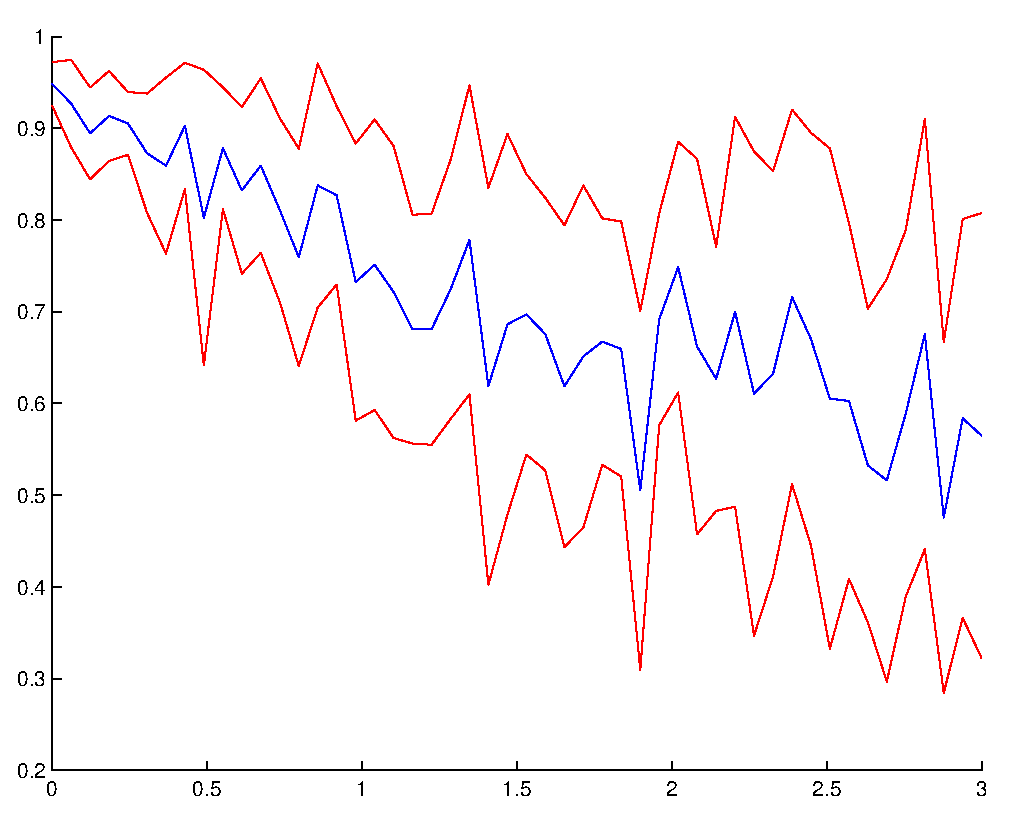
\includegraphics[width=65mm]{matlab/figura/iris_BAYES_ParzenSearch.eps} &
% 	  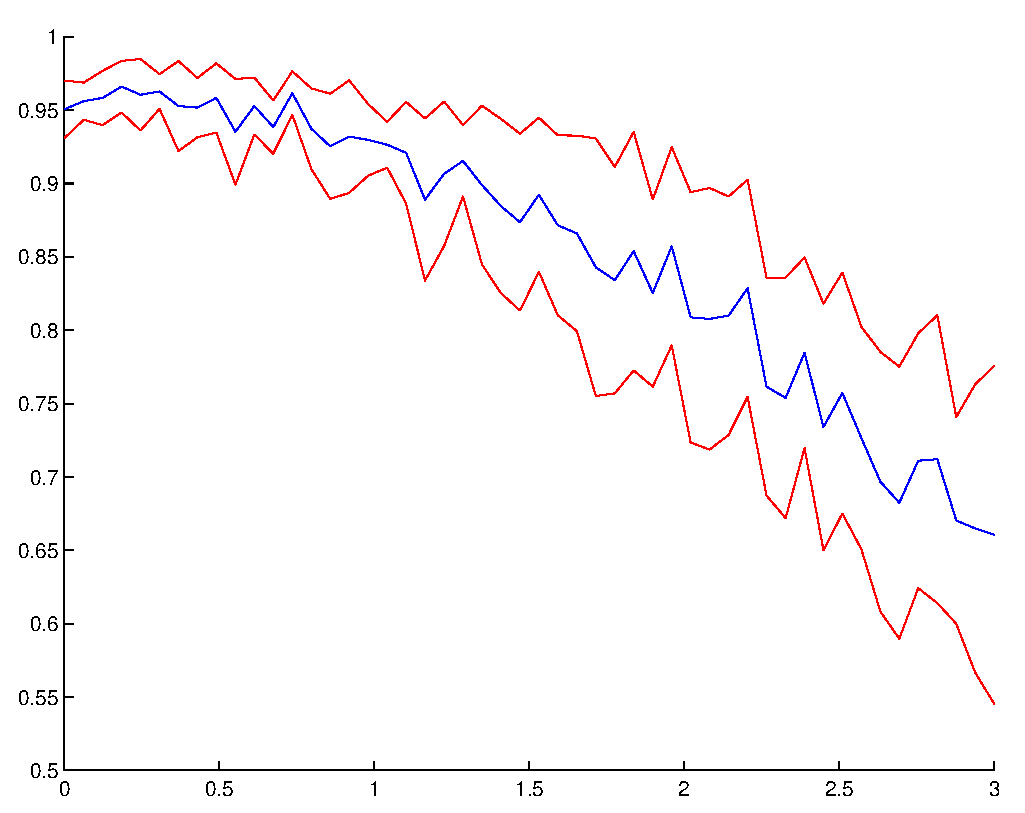
\includegraphics[width=65mm]{matlab/figura/derme_BAYES_ParzenSearch.eps}
% 	  \\
% 	(a) Íris & (b) Dermatologia \\[6pt] 
% 	 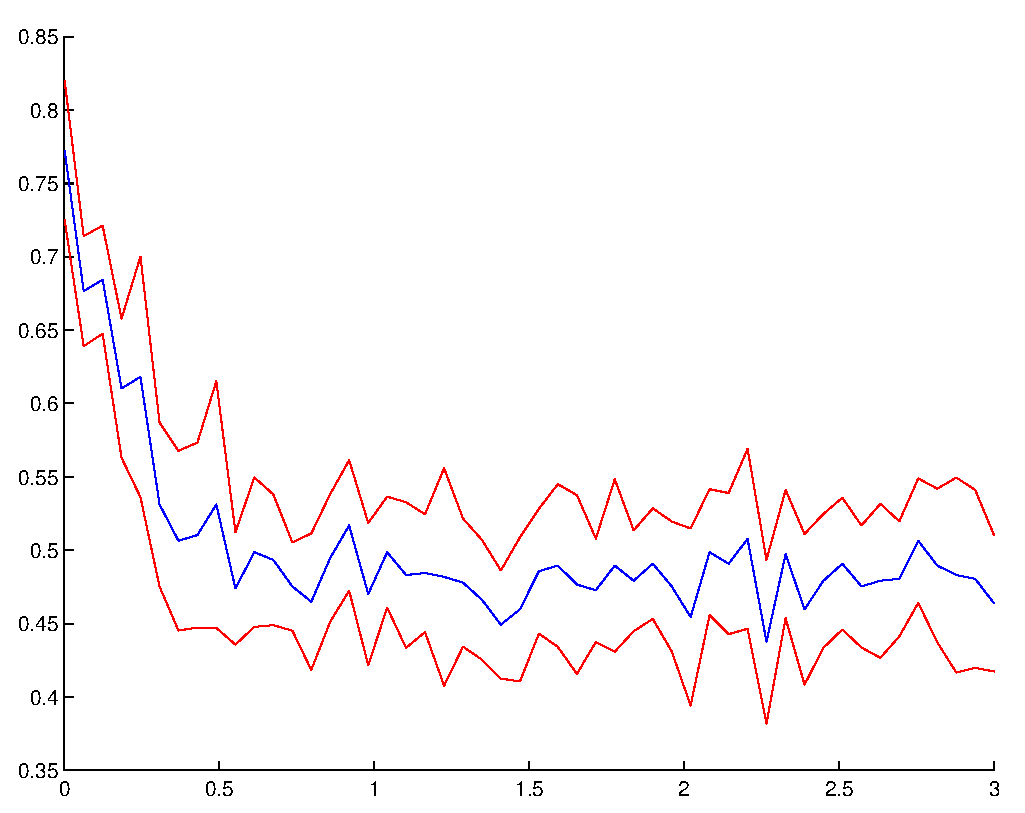
\includegraphics[width=65mm]{matlab/figura/vertebra_BAYES_ParzenSearch.eps}  &
% 	 \\
% 	 %\includegraphics[width=70mm]{matlab/figura/iris_KNN_RegDec_K75_1_3.eps} \\
% 	(c) Coluna Vertebral &  \\[6pt] 
% 
% 	\end{tabular}
% 
% 	\caption{Resultados da busca pela largura ótima da janela de parzen.}
% 	\label{fig:parzenGraphResults}
% \end{figure}
% 
% 
% 


\subsection{Análise da região de decisão}
Abaixo são apresentadas as regiões de decisões obtidas para os 3 problemas,
íris, vertebra e dermatologia. 

Para o problema da íris as regiões de decisões foram calculadas utilizandos os
atributos largura da pétala x comprimento da pétala e largura da sépala x
comprimento da pétala.

Para o problema da coluna vertebral as regiões de decisões foram calculadas
utilizandos os atributos pelvic incidence x pelvic tilt e pelvic incidence x
sacral slope.

Para o problema da dermatologia as regiões de decisões foram calculadas
utilizandos os atributos erythema x exocytosis e erythema x
acanthosis.

\subsubsection{ Gaussiana como PDF e matrizes de covariância distintas.
$\Sigma_i \neq \Sigma_j \forall i \neq j $ } Com matrizes de covariâncias distintas temos uma região de
decisão quadrática desta forma podemos notar várias elipses ao longo das
regiões, figura \ref{fig:regiaoGauss}. Podemos perceber na terceira coluna como
os dados foram classificados sobre a região de decisão. Poucas amostras foram
classificadas de forma errada, em especial para a base da íris. Já para a base
da dermatologia o número de amostras erradas foi ligeiramente maior.

\begin{figure}
	\centering
	\begin{tabular}{ccc}
	  \multicolumn{3}{c}{Íris}\\
	  %Íris
	  \includegraphics[width=40mm]{matlab/figura/gauss/iris/iris_BAYES_BayesDecP1_3_4.eps}
	  &
	  \includegraphics[width=40mm]{matlab/figura/gauss/iris/iris_BAYES_BayesDecP2_3_4.eps}
	  &
	  \includegraphics[width=40mm]{matlab/figura/gauss/iris/iris_BAYES_RegDec_3_4.eps}
	  \\
	  
	  \includegraphics[width=40mm]{matlab/figura/gauss/iris/iris_BAYES_BayesDecP1_1_4.eps}
	  &
	  \includegraphics[width=40mm]{matlab/figura/gauss/iris/iris_BAYES_BayesDecP2_1_4.eps}
	  &
	  \includegraphics[width=40mm]{matlab/figura/gauss/iris/iris_BAYES_RegDec_1_4.eps}
	  \\
	  %%-----------------------------------------------------------------------------------
	  % Dermatologia
	  \multicolumn{3}{c}{Dermatologia}\\
      \includegraphics[width=40mm]{matlab/figura/gauss/derme/derme_BAYES_BayesDecP1_1_16.eps}
      &
	  \includegraphics[width=40mm]{matlab/figura/gauss/derme/derme_BAYES_BayesDecP2_1_16.eps}
	  &
	  \includegraphics[width=40mm]{matlab/figura/gauss/derme/derme_BAYES_RegDec_1_16.eps}
	  \\	  
	  
      \includegraphics[width=40mm]{matlab/figura/gauss/derme/derme_BAYES_BayesDecP1_1_17.eps}
      &
	  \includegraphics[width=40mm]{matlab/figura/gauss/derme/derme_BAYES_BayesDecP2_1_17.eps}
	  &
	  \includegraphics[width=40mm]{matlab/figura/gauss/derme/derme_BAYES_RegDec_1_17.eps}
	  \\	
	  %%-----------------------------------------------------------------------------------
	  % Coluna
	  \multicolumn{3}{c}{Coluna Vertebral}\\
      \includegraphics[width=40mm]{matlab/figura/gauss/vertebra/vertebra_BAYES_BayesDecP1_1_2.eps}
      &
	  \includegraphics[width=40mm]{matlab/figura/gauss/vertebra/vertebra_BAYES_BayesDecP2_1_2.eps}
	  &
	  \includegraphics[width=40mm]{matlab/figura/gauss/vertebra/vertebra_BAYES_RegDec_1_2.eps}
	  \\	  
	  
      \includegraphics[width=40mm]{matlab/figura/gauss/vertebra/vertebra_BAYES_BayesDecP1_1_5.eps}
      &
	  \includegraphics[width=40mm]{matlab/figura/gauss/vertebra/vertebra_BAYES_BayesDecP2_1_5.eps}
	  &
	  \includegraphics[width=40mm]{matlab/figura/gauss/vertebra/vertebra_BAYES_RegDec_1_5.eps}
	  \\		  	  
	 \multicolumn{1}{p{40mm}}{(a) $P(W_i|x)$}
	 &
	 \multicolumn{1}{p{40mm}}{(b) Regiao de decisão}
	 &
	 \multicolumn{1}{p{40mm}}{(c) Resultado
	 da classificação dos dados sobre a regiao de decisão}
	 
	\end{tabular}
	\caption{Resultados utilizando matrizes de covariâncias distintas.}
	\label{fig:regiaoGauss}
\end{figure}





% 
% 
% \subsection{PDF Janela de Parzen}
% Abaixo é apresentado o resultado da segmentação de uma imagem utilizando o
% classificador Bayessiano, desta vez utilizando janela de parzen como função de
% densidade probabilidade. Foram realizados três testes com três variancias da
% janela, valor de h, distintas. Os valores testados foram, 0.05, 0.5 e 1. Com o
% aumento do valor de h houve uma maior suavização
% 
% 
% \begin{figure}
% 	\centering
% 	\begin{tabular}{cc}
% 	  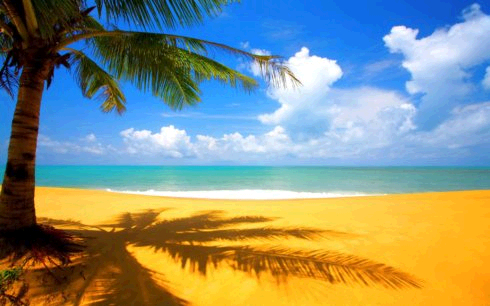
\includegraphics[width=45mm]{matlab/figura/gauss/segmentacao/paradise.jpg} & 
% 	  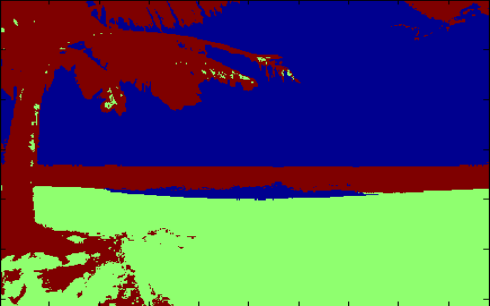
\includegraphics[width=45mm]{matlab/figura/parzen/segmentacao/paradiseRes.png}
% 	  \\ 
% 	  (a) Original & (b) h=0.05\\
% 	  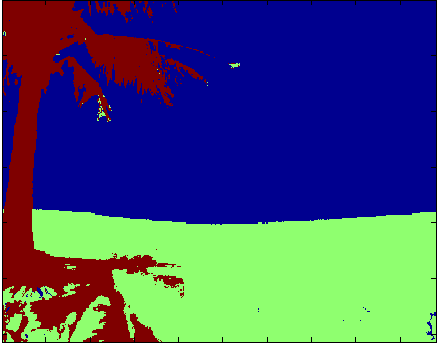
\includegraphics[width=45mm]{matlab/figura/parzen/segmentacao/paradiseRes05.png} & 
% 	  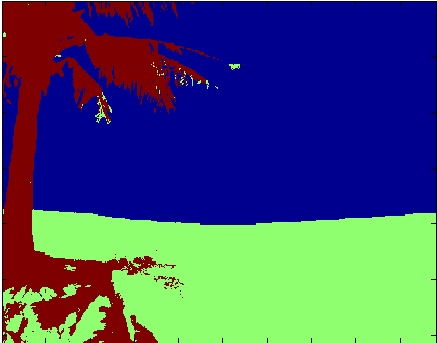
\includegraphics[width=45mm]{matlab/figura/parzen/segmentacao/paradiseRes1.png}
% 	   \\
% 	  (c) h=0.5 & (d) h=1\\
% 	\end{tabular}
% 	\caption{Resultado da segmentação utilizando o classificador Bayessiano com
% 	janela de parzen.
% 	Com o aumento do valor de h pode-se notar que a segmentação se torna mais
% 	suave.}
% 	\label{fig:resultGaussSegParadise}
% \end{figure}
% 


\bookmarksetup{startatroot}% 
% ---

% ---
% Conclusão
% ---

\section*{Considerações finais}




\addcontentsline{toc}{section}{Considerações finais}
Neste trabalho foram apresentados os resultados obtidos ao testar várias funções
de densidade de probabilidade junto ao classificador bayessiano. Os resultados
podem ser visualizados na tabela \ref{tab:acuracia}. Podemos observar uma
superioridade dos métodos não lineares frente aos lineares, bem como uma maior
acurácia para métodos que consideram melhor a modelagem dos dados, quando se
utiliza matrizes de covariância diferentes para cada classe de problema.


% ----------------------------------------------------------
% ELEMENTOS PÓS-TEXTUAIS
% ----------------------------------------------------------
\postextual

% ----------------------------------------------------------
% Referências bibliográficas
% ----------------------------------------------------------
%\bibliography{bib,iris}

% ----------------------------------------------------------
% Glossário
% ------------------------------------ ----------------------
%
% Há diversas soluções prontas para glossário em LaTeX. 
% Consulte o manual do abnTeX2 para obter sugestões.
% 
%\glossary 

% ----------------------------------------------------------
% Apêndices
% ----------------------------------------------------------


\end{document}